\section{User interface}

\subsection{Structure}

A small overview of the menu Structure.

\subsubsection{Start screen}
The Start screen will be shown when the app is launched, can switch to everything. He can enter the VR-Mode, Live-Data from the sensor or change the settings.

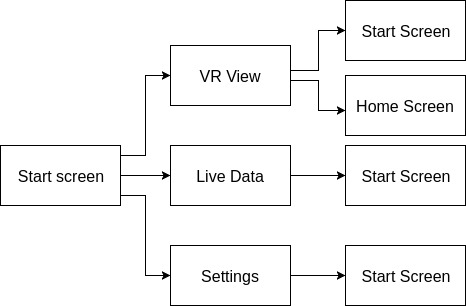
\includegraphics[scale=0.5]{pics/startscreen.jpg}

\subsubsection{VR-Mode}

The VR-Mode launches normally in normal 3D mode from where the user can switch to stereoscopic 3D view by touching the button in the lower left corner or by pressing the A-Button on his controller.

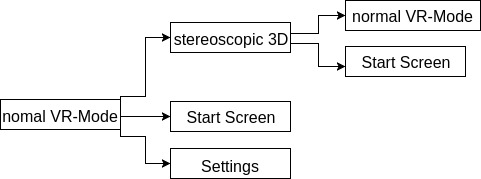
\includegraphics[scale=0.5]{pics/Vr-Mode.jpg}


\subsubsection{Live Data}
Live Data just shows the current live data from the connected sensor.

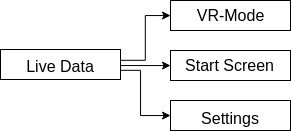
\includegraphics[scale=0.5]{pics/Live_Data.jpg}

\newpage

\subsubsection{Settings}

Here the user can select which sensor in range he wants to connect to and some basic settings like switching blue-tooth on and scan for more devices.
From the Setting menu the user can switch to VR-Mode without going back to the start screen.

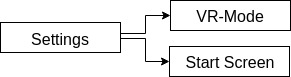
\includegraphics[scale=0.5]{pics/Settings.jpg}

\subsection{Layout}

A mockup of the Start up screen. 
\\
\\
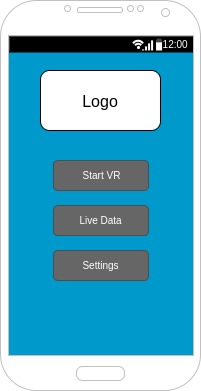
\includegraphics[scale=0.5]{pics/startScreen_mockup.jpg}
\\

And a mockup of the stereoscopic Vr-Mode.
\\
\\
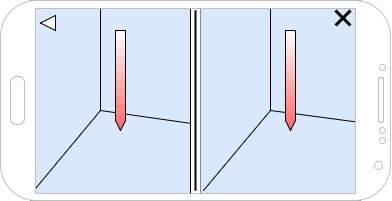
\includegraphics[scale=0.5]{pics/VRView_mockup.jpg}
